\documentclass{article}

\usepackage{graphicx}
\usepackage[letterpaper,margin=1in]{geometry}
\usepackage{hyperref}
\usepackage{url}
\usepackage{verbatim}
\usepackage{caption}

\hypersetup{colorlinks=true,urlcolor=blue}

\title{Deterministic aggregate generation program}
\author{Egor Demidov}

\begin{document}
\maketitle

\section*{Synopsis}

This program can generate different types of deterministic fractal aggregates, including several types of named aggregates. The fractal (Hausdorff) dimesion of those aggregates is well-known and the size can be controlled by adjusting the ``number of iterations'' parameter.

\section*{Compilation}

A modern C++ compiler is required to build the program. The use of CMake is recommended to generate build files. This program depends on libFractalCommon, which is available at \href{https://github.com/eg0000r-pub/libFractalCommon}{https://github.com/eg0000r-pub/libFractalCommon}.

In \texttt{CMakeLists.txt} change the line \path{include_directories("/home/egor/Libraries/include")} to the path where the libFractalCommon headers are stored and change the line \path{link_directories("/home/egor/Libraries/bin")} to the path where libFractalCommon binary is stored. Now in the folder with the sources execute the following commands:

\begin{verbatim}
mkdir cmake-build
cd cmake-build
cmake -DCMAKE_BUILD_TYPE=Release ..
cmake --build .
\end{verbatim}

An executable file named \texttt{deterministic\_aggregates} will appear in the \texttt{cmake-build} directory. Run the program with \texttt{./deterministic\_aggregates}.

\section*{Usage}

When the program is executed, the user will be prompted to enter the number of algorithm iterations, the output file name, and the aggregate type. The number of iterations parameter will affect the number of primary particles in the produced aggregate and can be estimated with the equations provided in the ``Aggregates'' section of this document. The output file is where the generated aggregate data will be stored. Generated aggregates are stored in ASCII vtk files and the \texttt{.vtk} extension will be appended to the file name is not provided already. The aggregate type parameter determines which aggregate from the ``Aggregates'' section will be generated.

\section*{Aggregates}

\subsection*{Type A aggregate}

Features:

\begin{itemize}
	\item Fractal dimension $D_f$ is $\log_{3}{9}=2$
	\item Size $N$ is $9^{n}$ at $n$ iterations
	\item PPs can be represented with spheres of unit radius
\end{itemize}

\begin{figure}[htp]
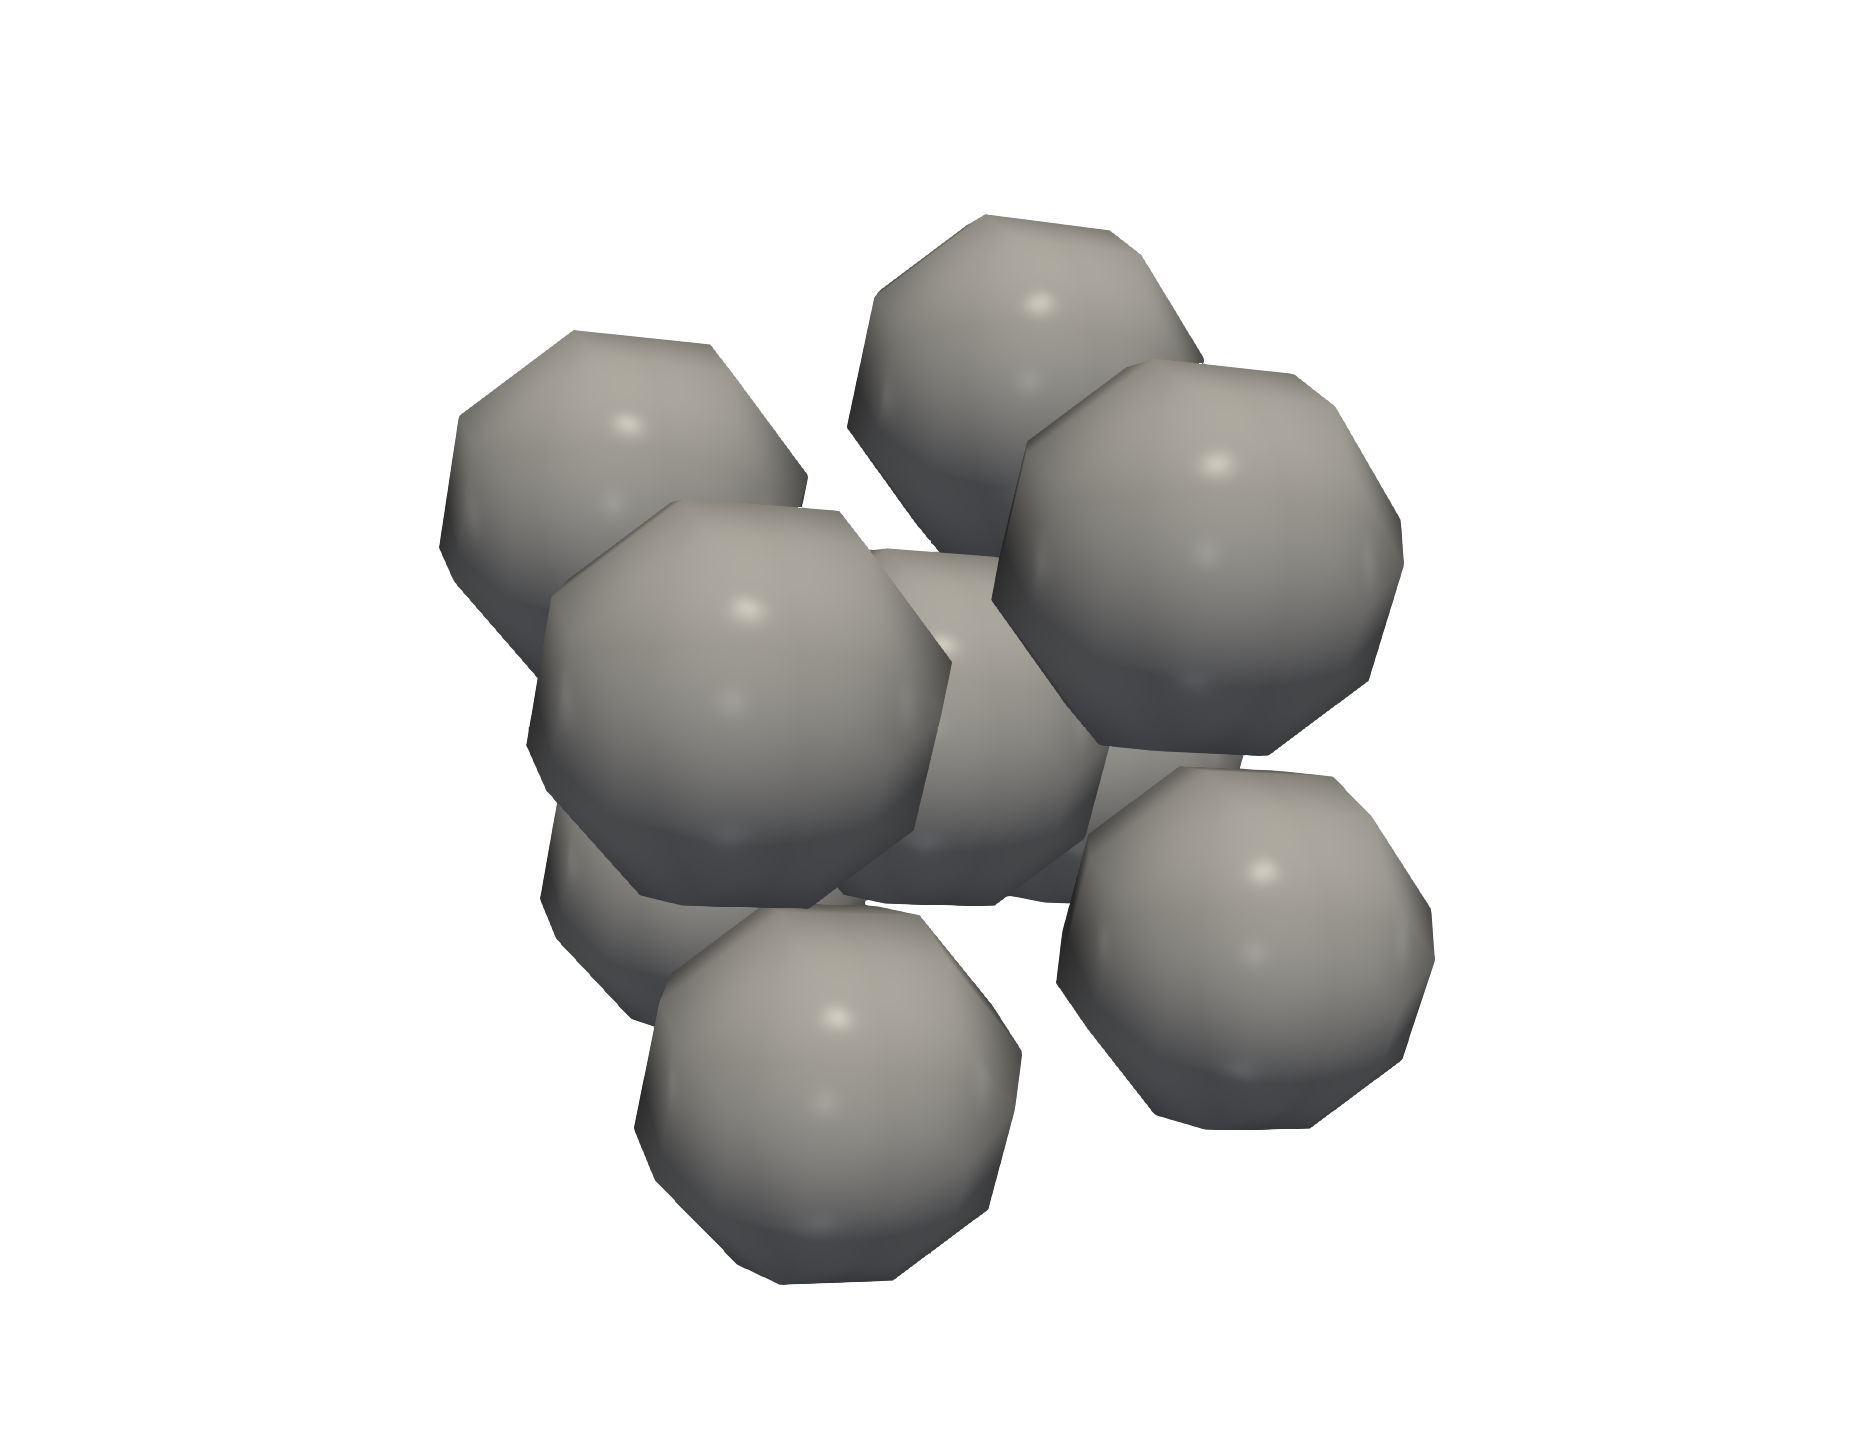
\includegraphics[width=0.49\textwidth]{resources/type-a-img-1.png}
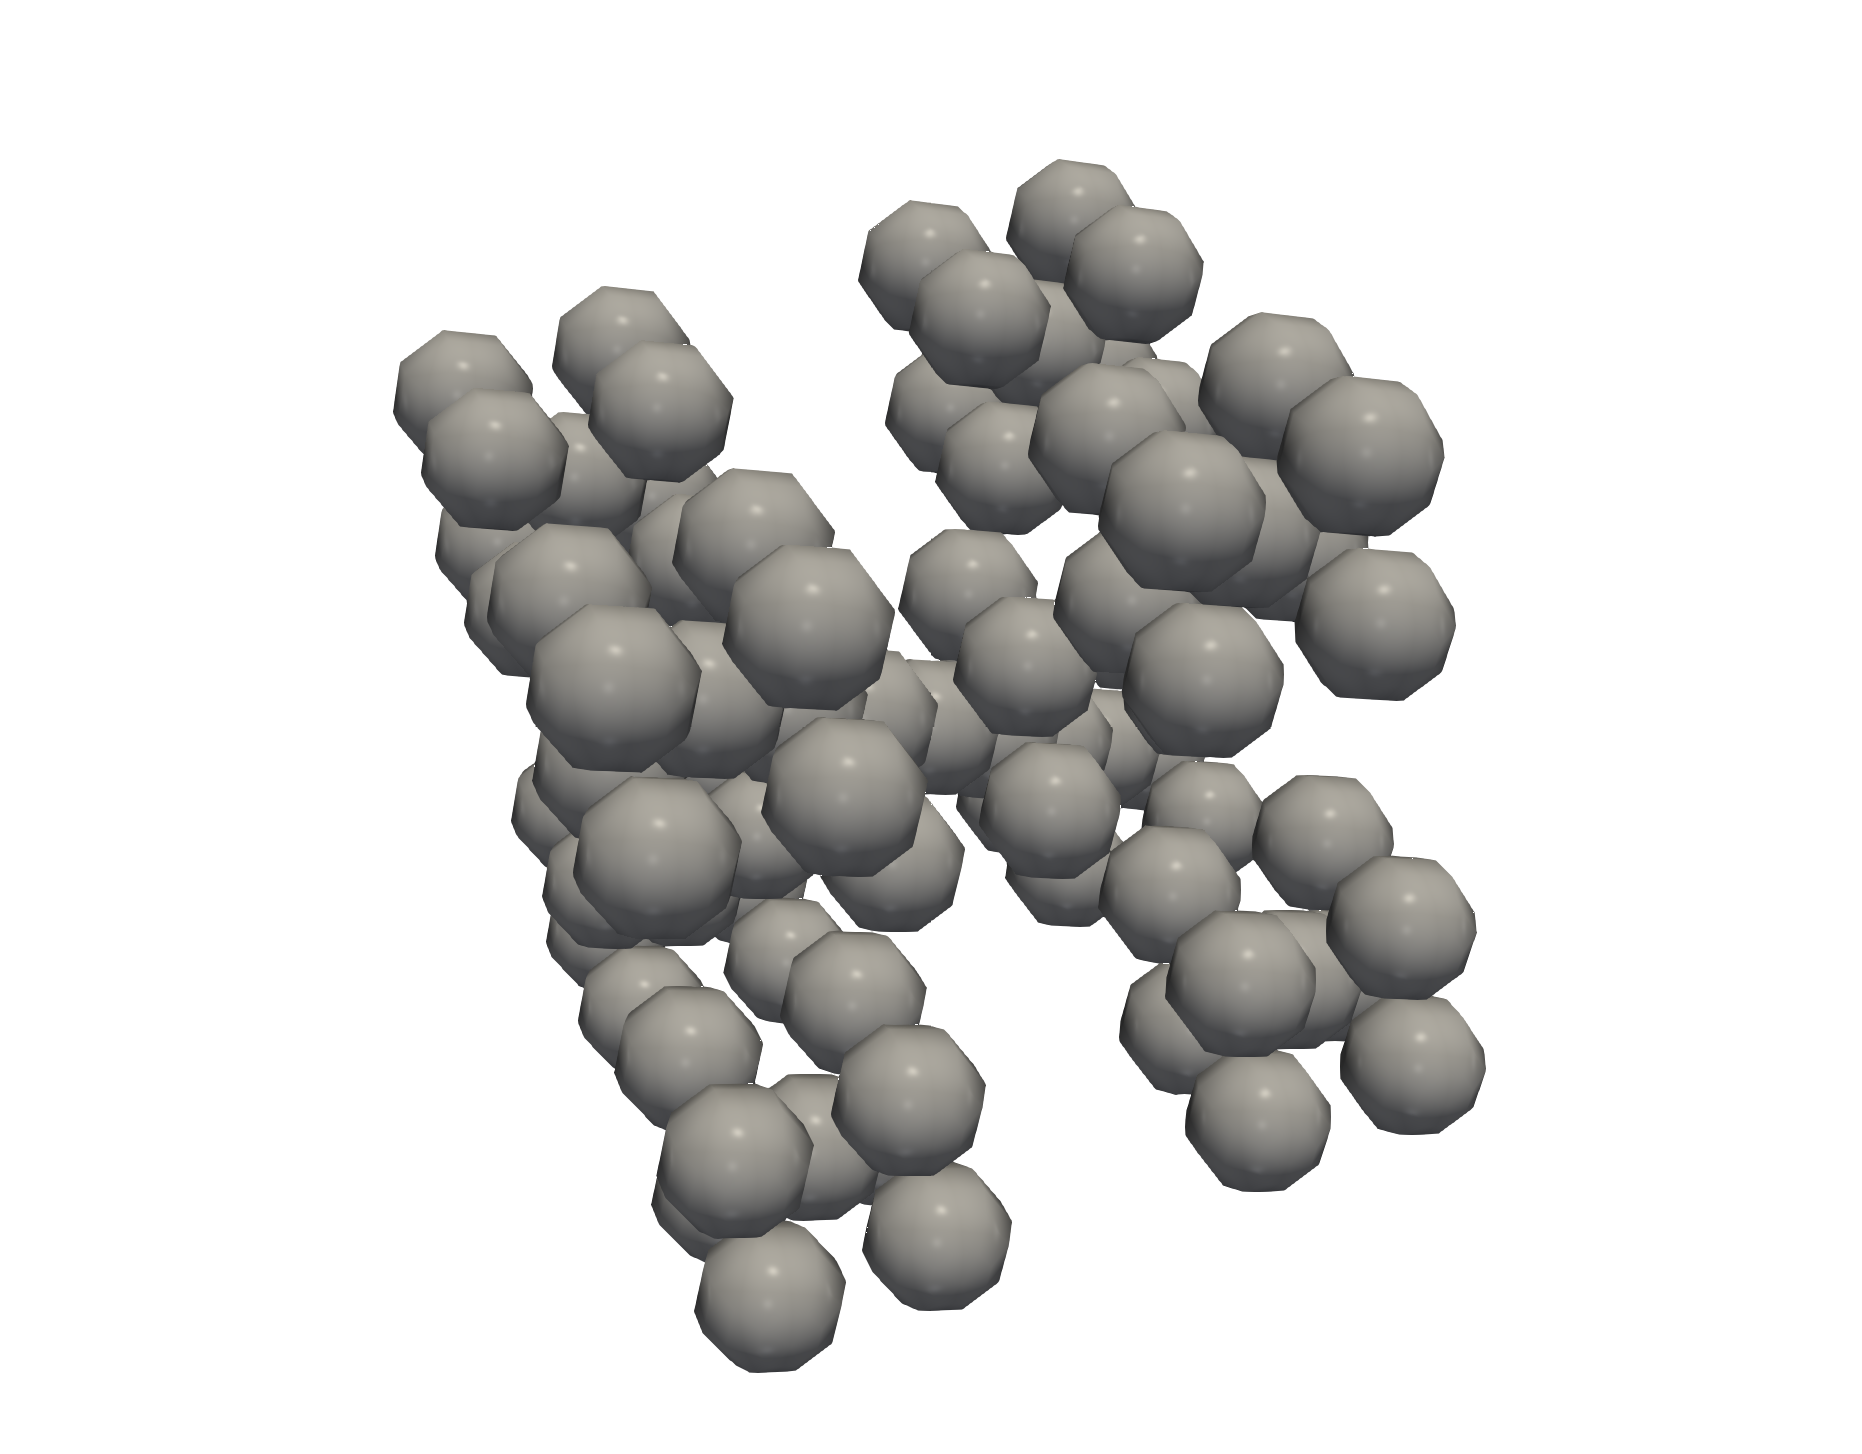
\includegraphics[width=0.49\textwidth]{resources/type-a-img-2.png}
\caption*{\underline{Type A} aggregate after 1 iteration (left) and 2 iterations (right)}
\end{figure}

\subsection*{Type B aggregate (a.k.a. 3D Vicsek fractal)}

Features:

\begin{itemize}
	\item Fractal dimension $D_f$ is $\log_{3}{7}=1.771$
	\item Size $N$ is $7^{n}$ at $n$ iterations
	\item PPs can be represented with spheres of unit radius or cubes of size 2
\end{itemize}

\begin{figure}[htp]
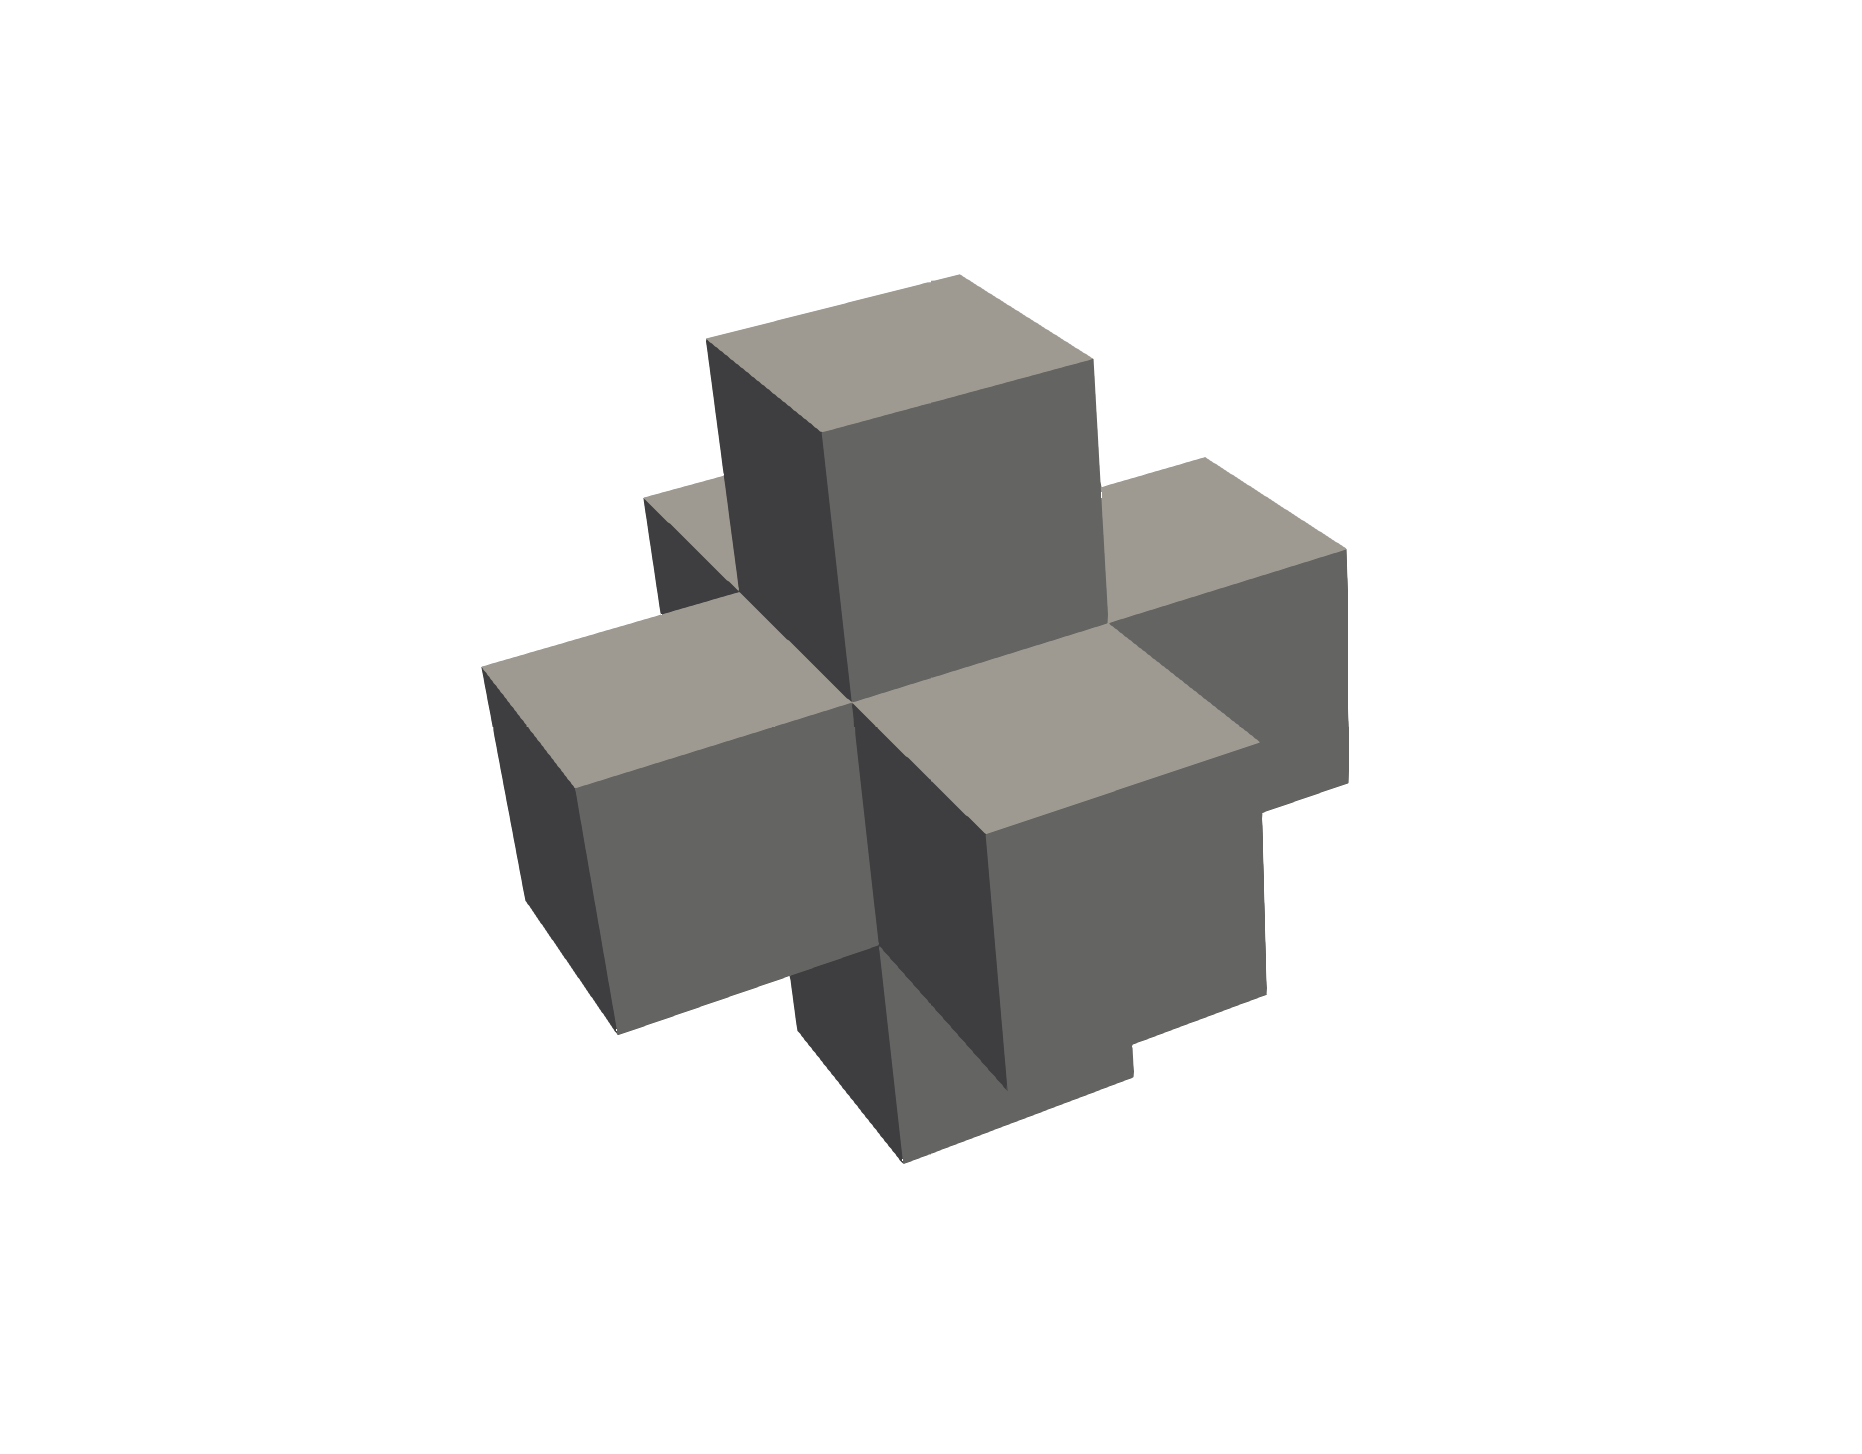
\includegraphics[width=0.49\textwidth]{resources/type-b-img-1.png}
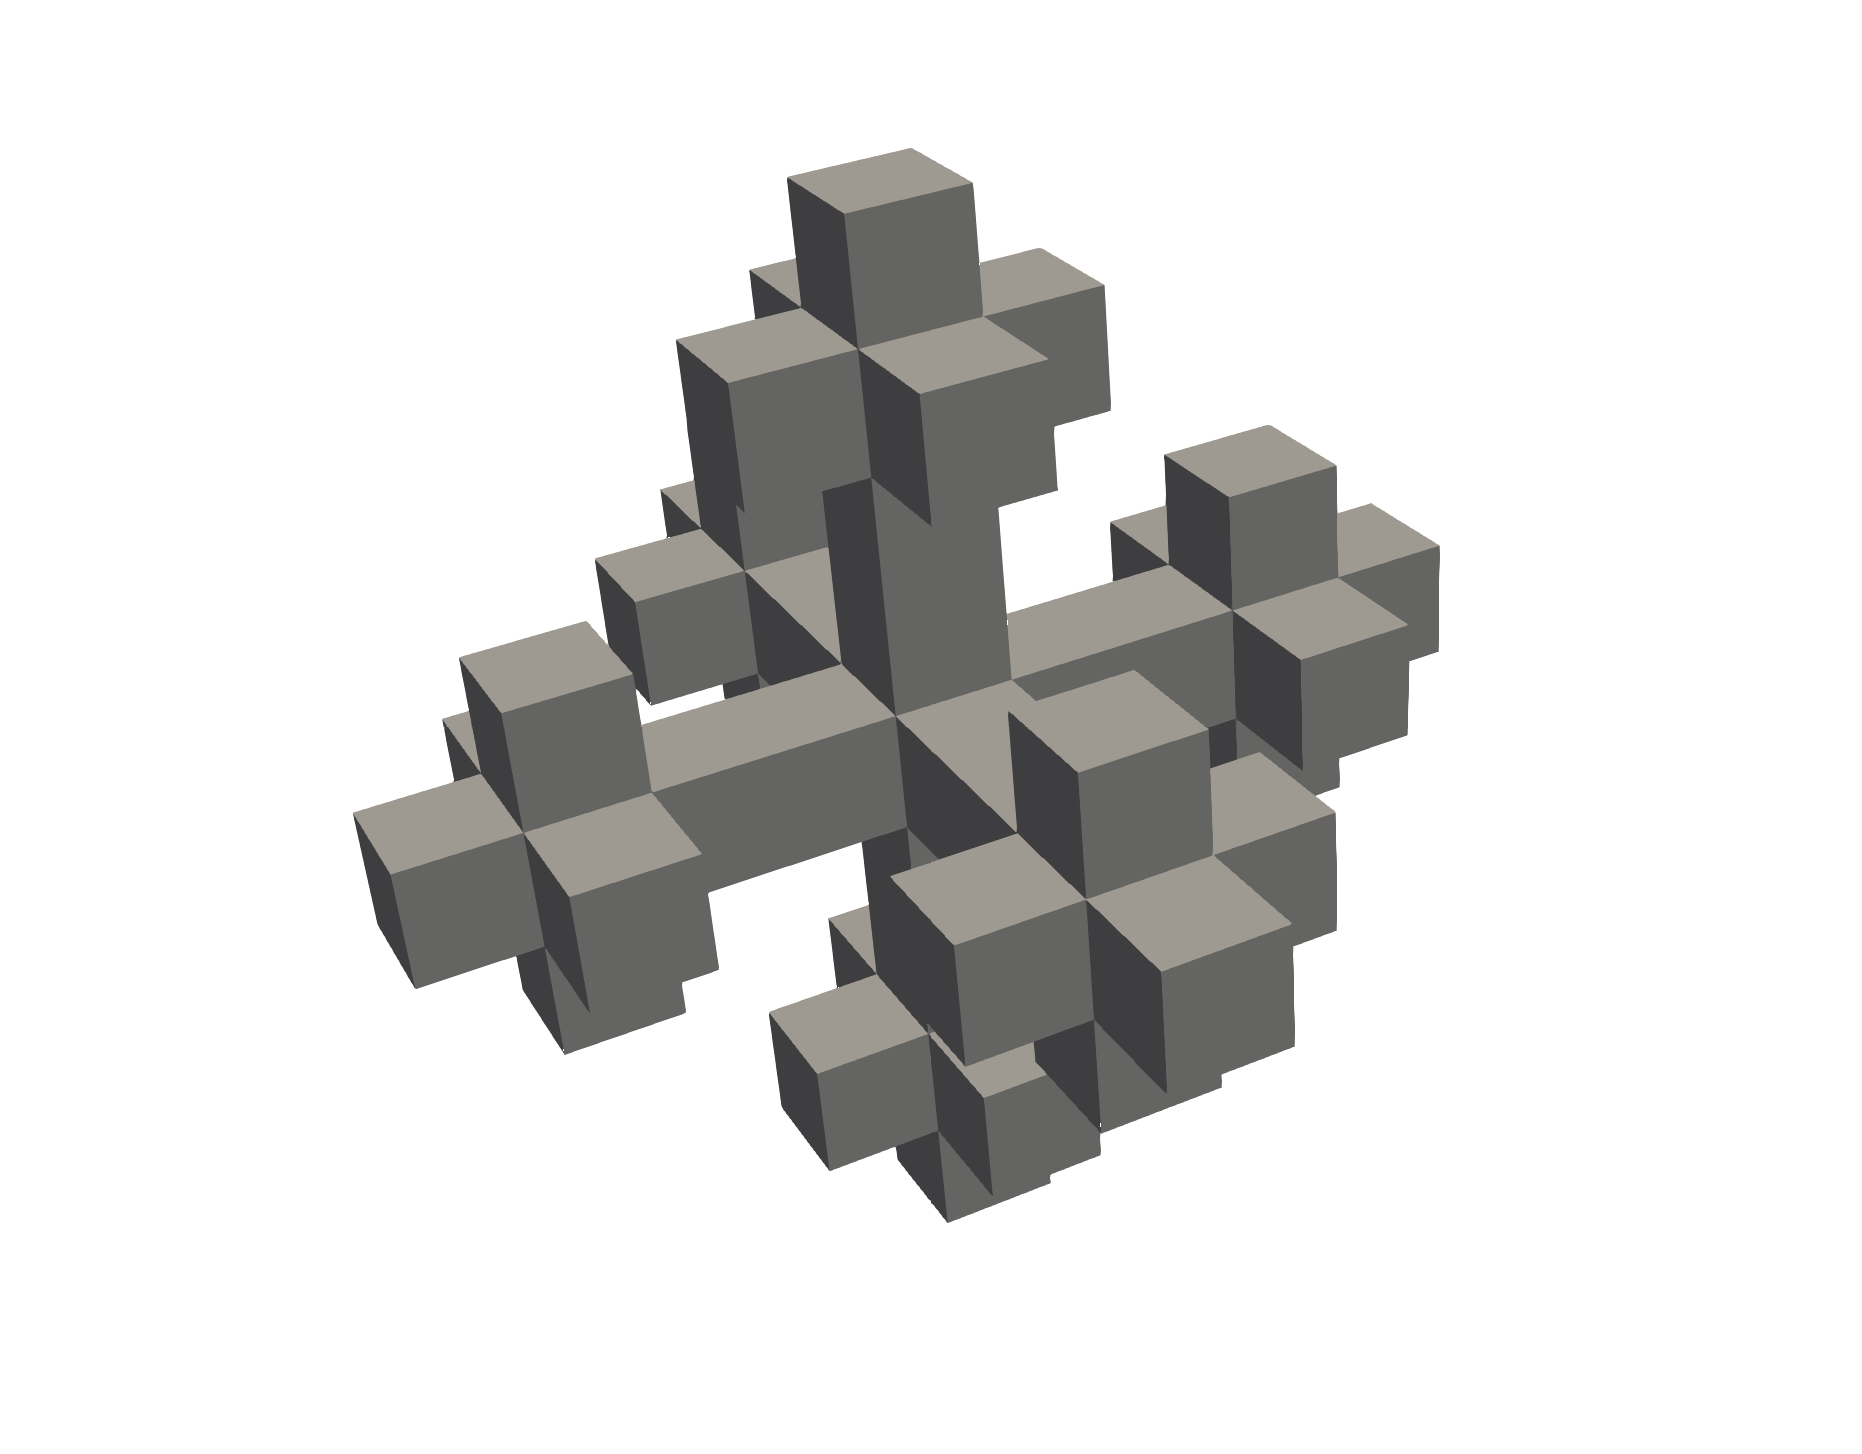
\includegraphics[width=0.49\textwidth]{resources/type-b-img-2.png}
\caption*{\underline{Type B} aggregate after 1 iteration (left) and 2 iterations (right)}
\end{figure}

\subsection*{Type C aggregate (a.k.a. Menger sponge)}

Features:

\begin{itemize}
	\item Fractal dimension $D_f$ is $\log_{3}{20}=2.727$
	\item Size $N$ is $20^{n+1}$ at $n$ iterations
	\item PPs can be represented with spheres of unit radius or cubes of size 2
\end{itemize}

\begin{figure}[htp]
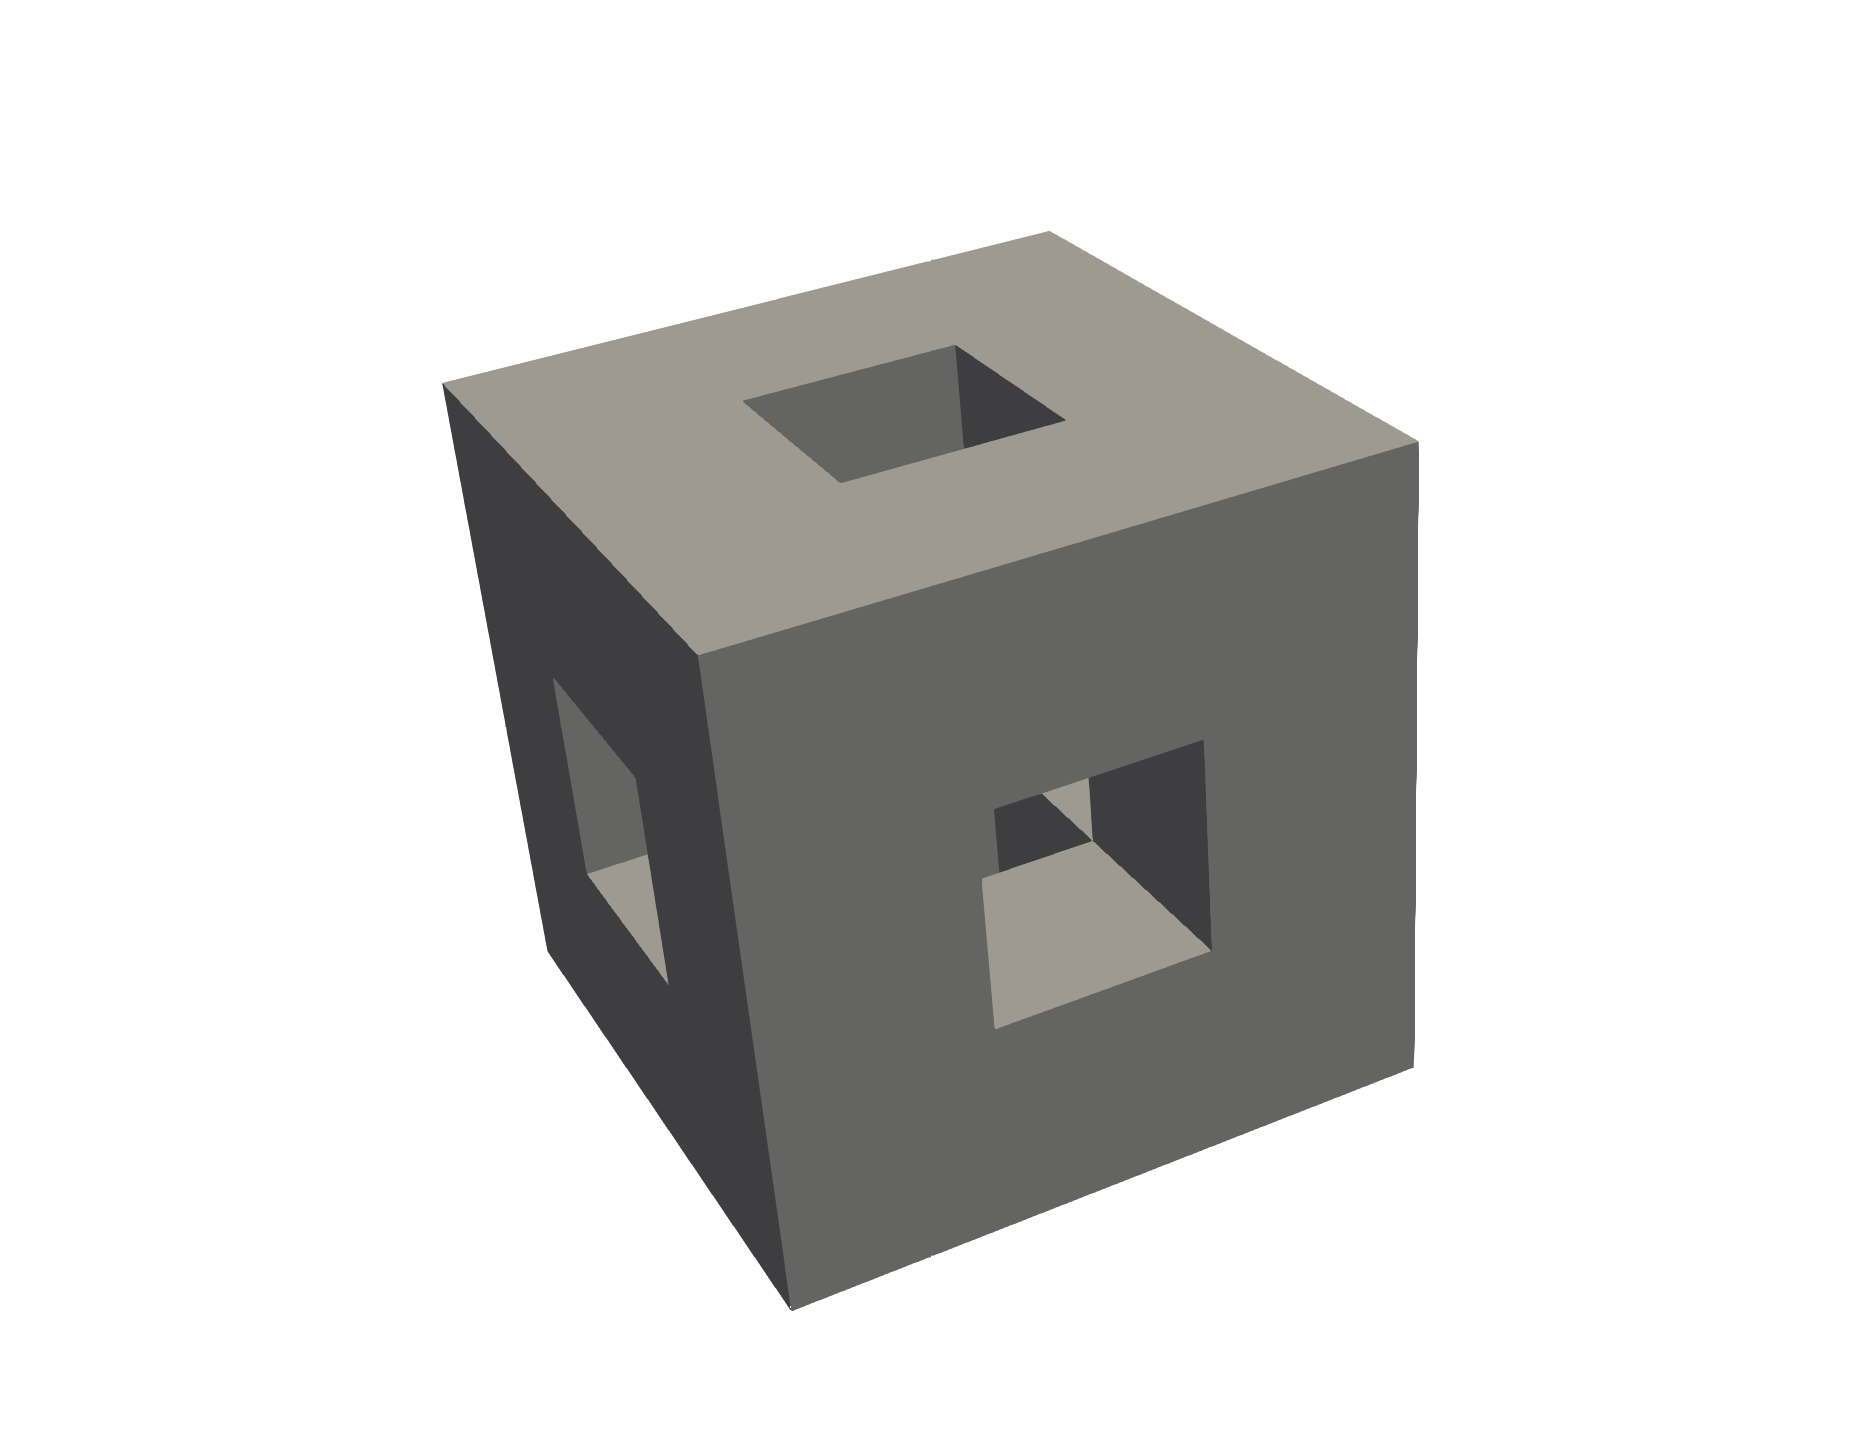
\includegraphics[width=0.49\textwidth]{resources/type-c-img-1.png}
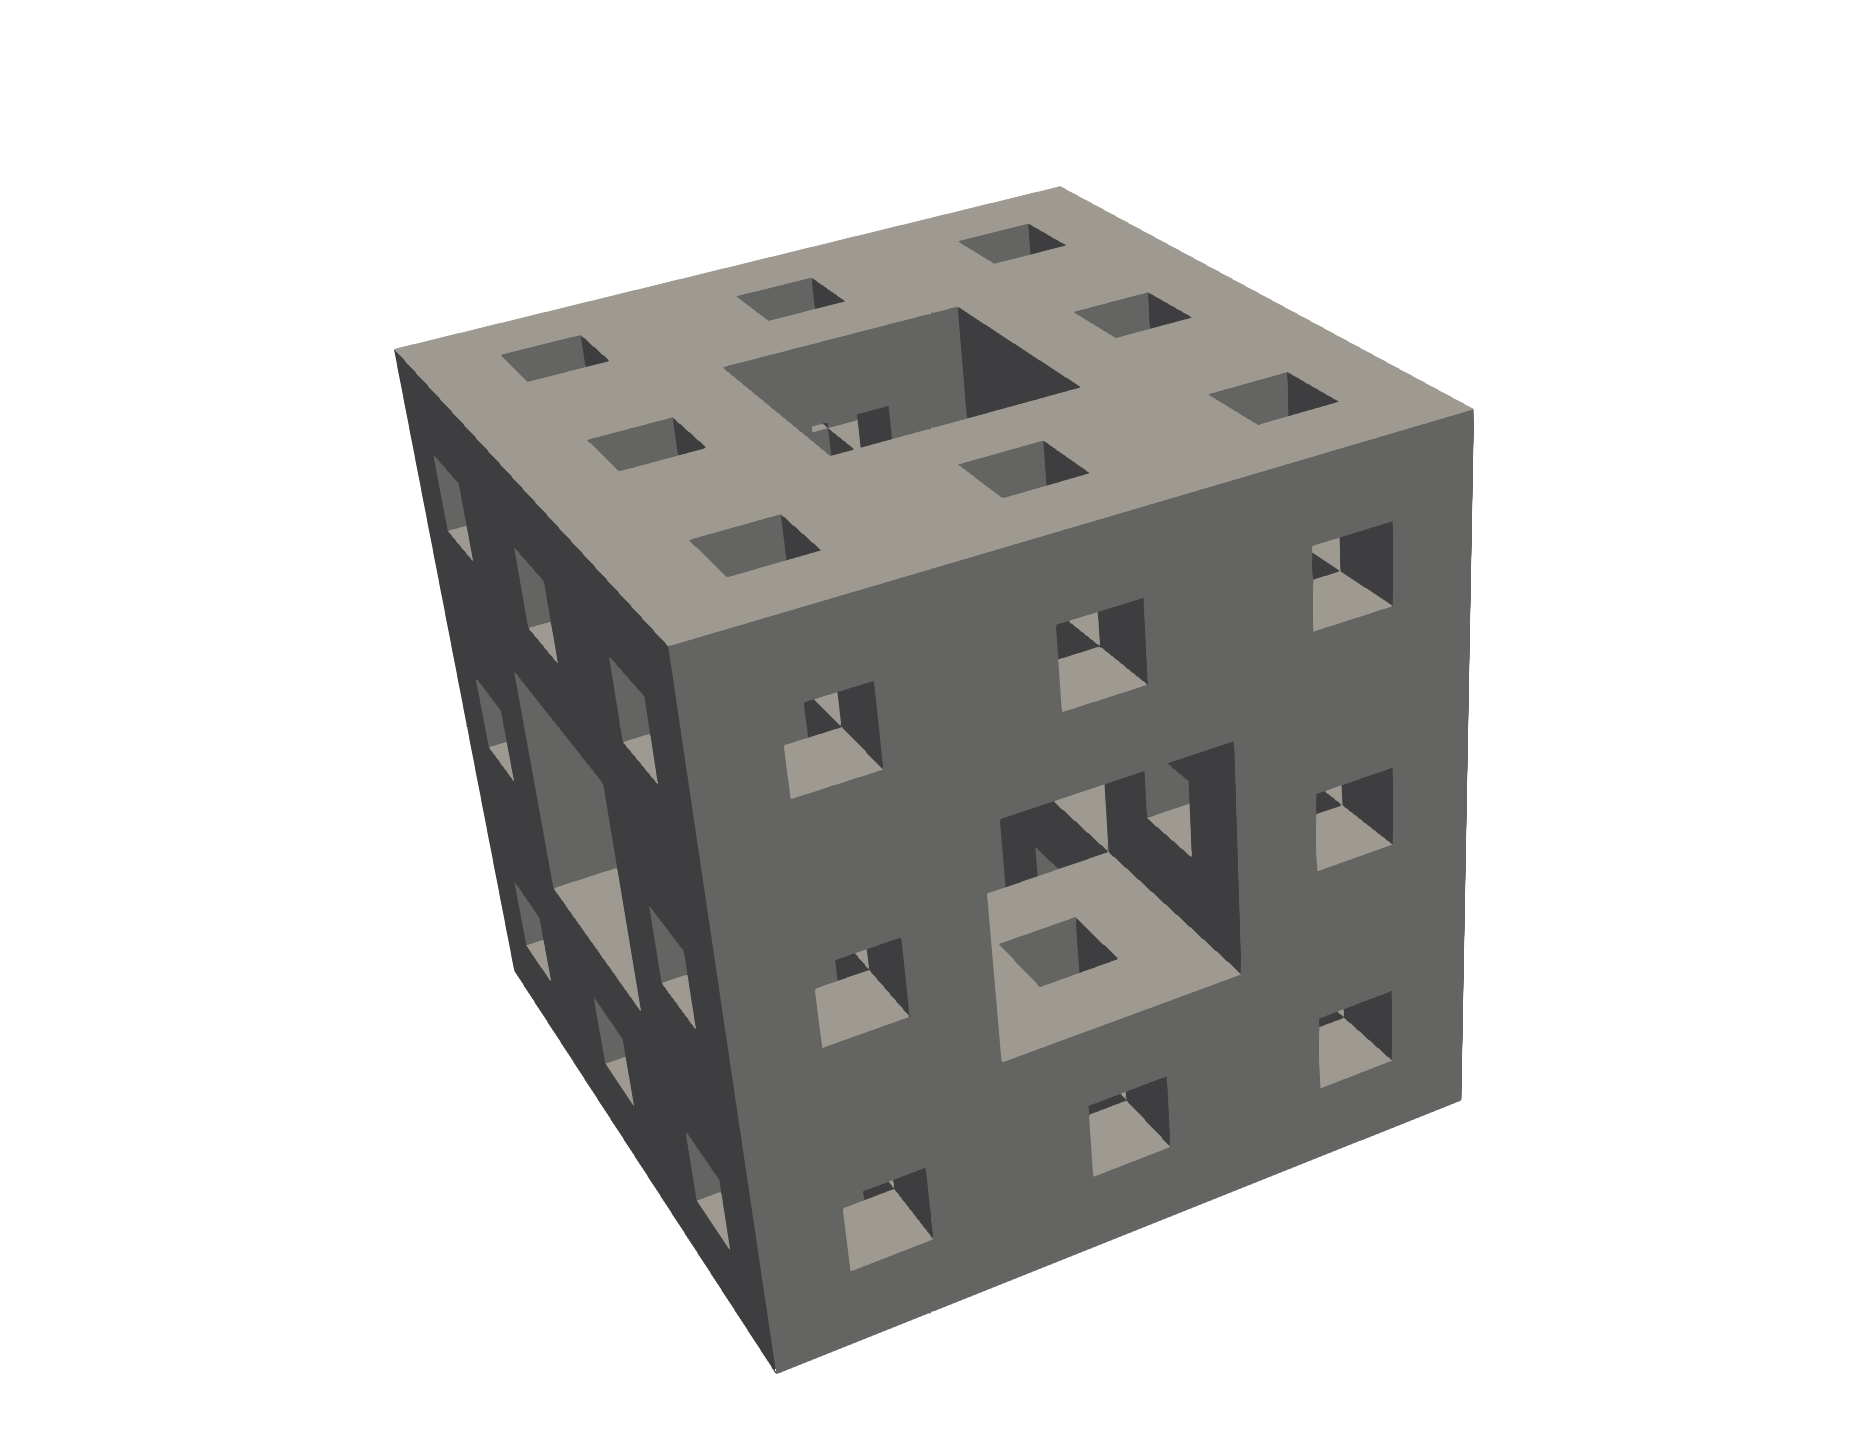
\includegraphics[width=0.49\textwidth]{resources/type-c-img-2.png}
\caption*{\underline{Type C} aggregate after 0 iterations (left) and 1 iteration (right)}
\end{figure}

\subsection*{Type D aggregate (a.k.a. Sierpinski pyramid)}

Features:

\begin{itemize}
	\item Fractal dimension $D_f$ is $\log_{2}{4}=2$
	\item Size $N$ is $4^{n+1}$ at $n$ iterations
	\item PPs can be represented with spheres of unit radius
\end{itemize}

\begin{figure}[htp]
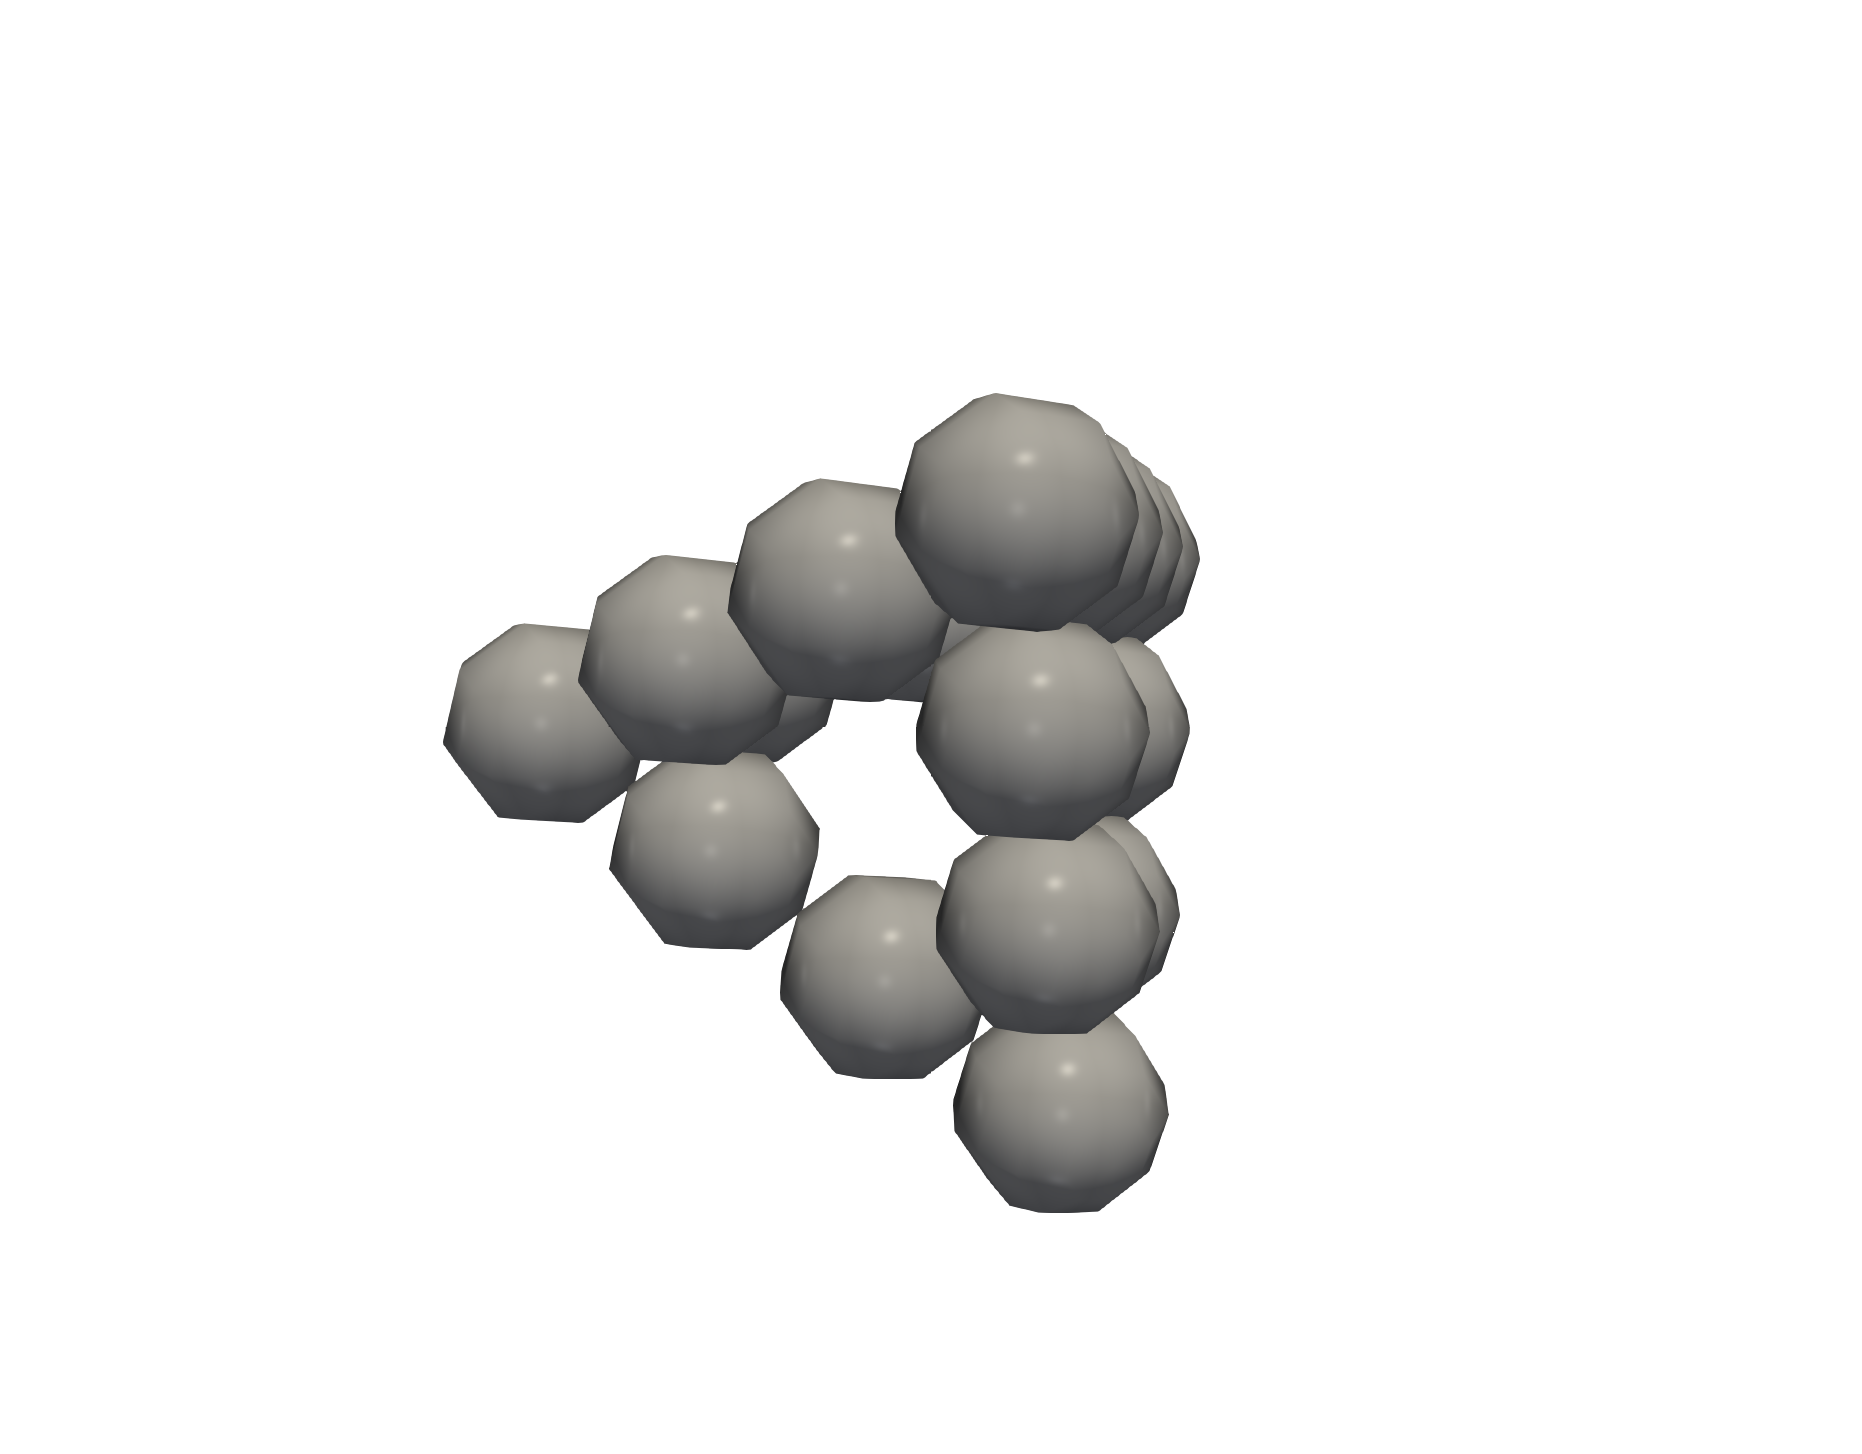
\includegraphics[width=0.49\textwidth]{resources/type-d-img-2.png}
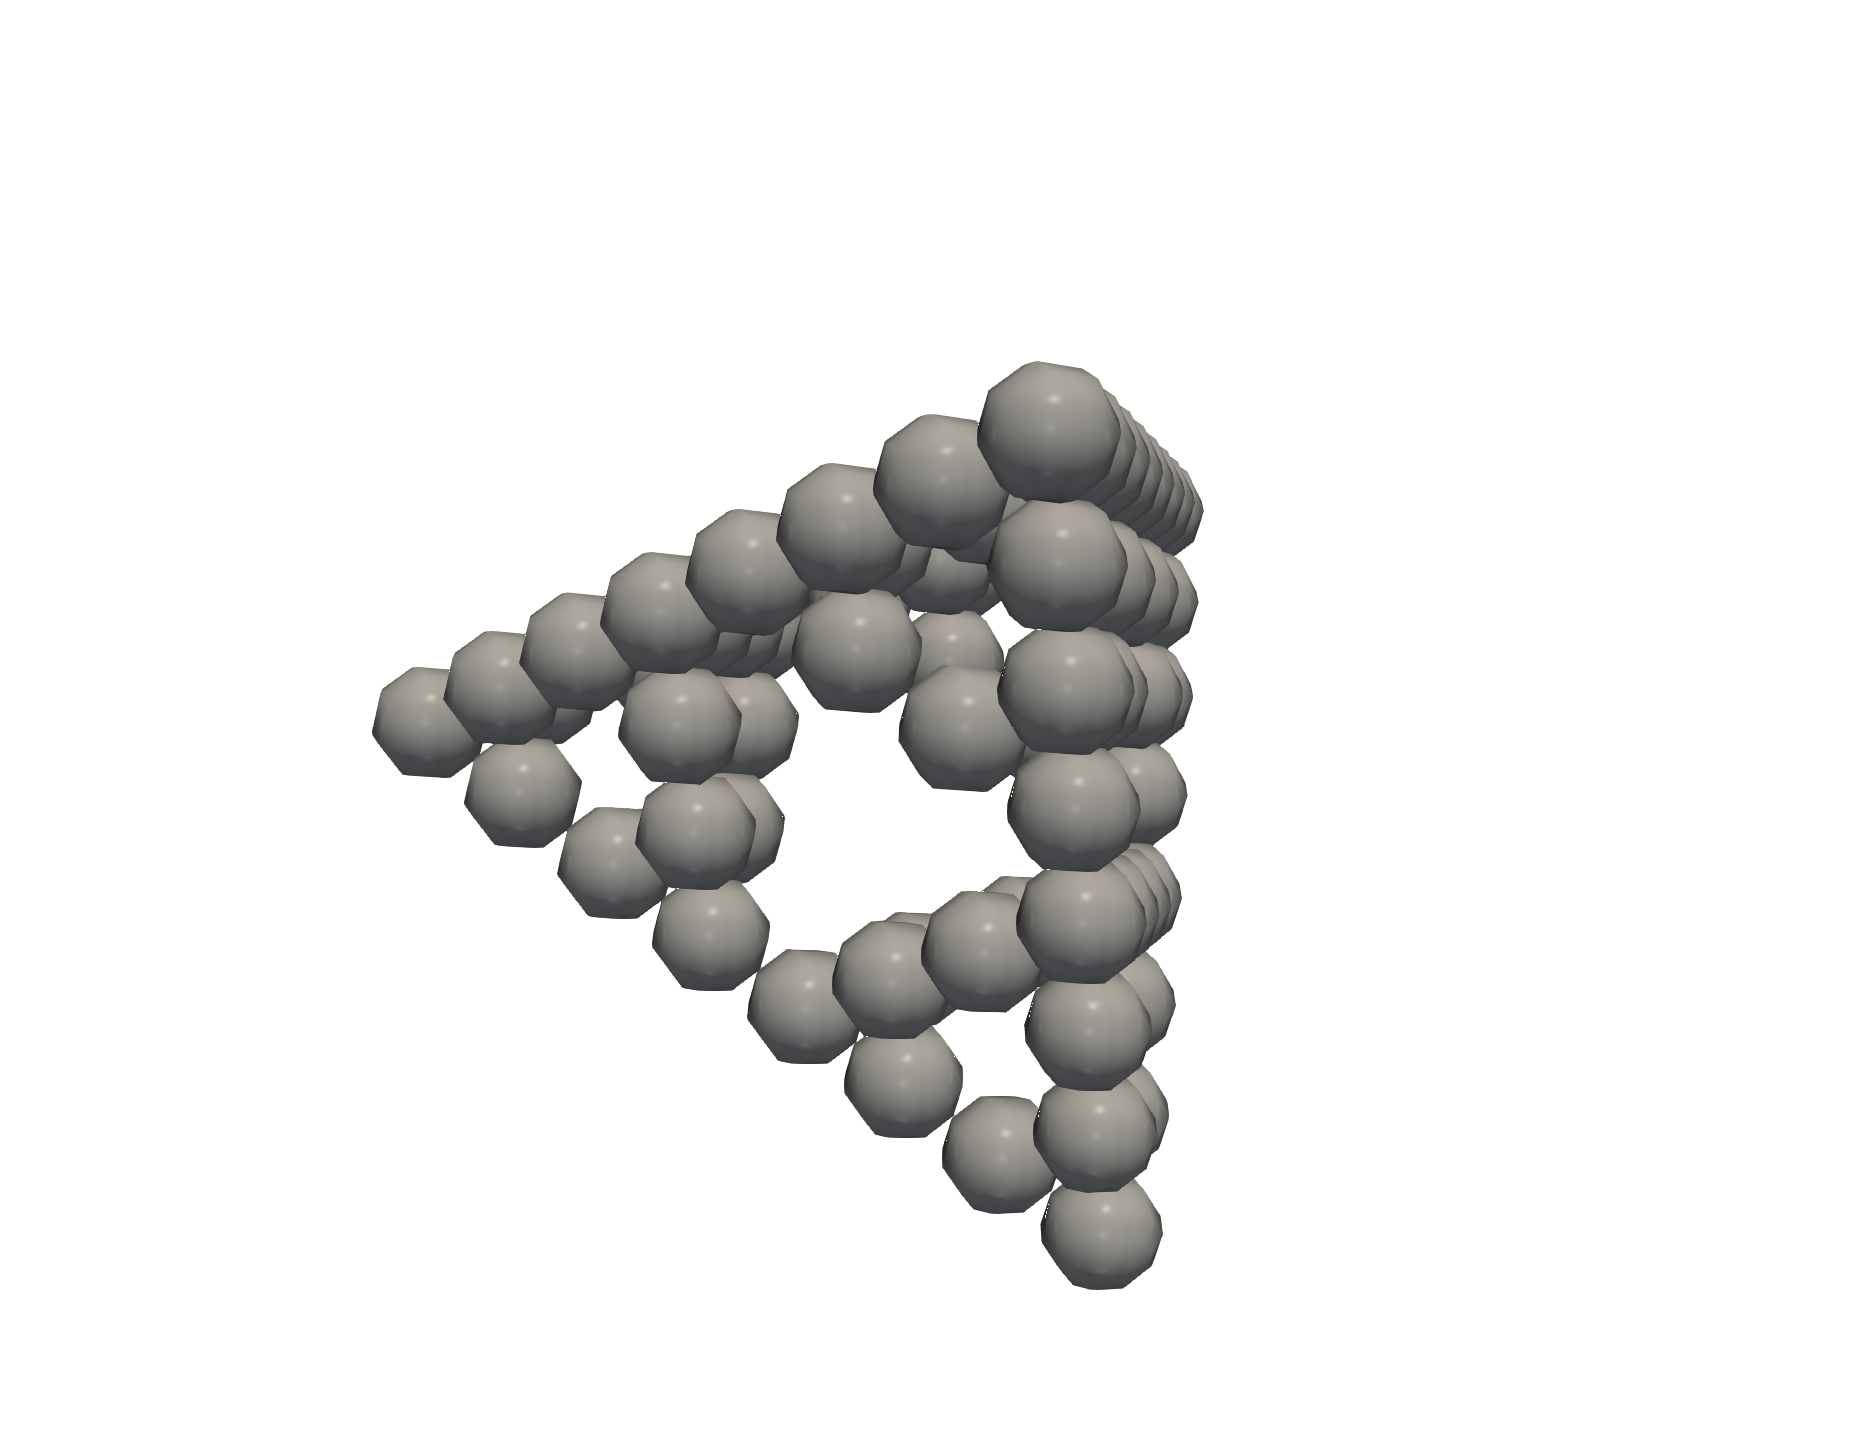
\includegraphics[width=0.49\textwidth]{resources/type-d-img-3.png}
\caption*{\underline{Type D} aggregate after 1 iteration (left) and 2 iterations (right)}
\end{figure}

\section*{Pre-exponential fractor}

Fractal dimesion can be derived from any property that is related to distribution of mass in space. One such property is radius of gyration ($R_g$) -- the root mean square distance of PPs from the center of mass of the aggregate. The center of mass $\vec{r}_o$ can be found with
$$
	\vec{r}_0=\frac{1}{N}\sum_{i=1}^{N}{\vec{r}_i}
$$
where $N$ is the number of PPs in the aggregate and $\vec{r}_i$ is postion of $i$-th PP. $R_g$ is then
$$
	R_g^2=\frac{1}{N}\sum_{i=1}^{N}{(\vec{r}_i-\vec{r}_0)^2}
$$
$N$ must be proportional to $R_g^{D_f}$. Let the proportionality constant be $k_0$, then
$$
	N=k_0(R_g)^{D_f}
$$
Knowing $N$, $D_f$, and $R_g$ for each aggregate type we can readily compute $k_0$. The calculated values are presented in the table below.

\begin{table}[htp]
\centering
\begin{tabular}{c c}
\hline
	Type & $k_0$\\
\hline
	A & 2.25\\
	B & 2.12\\
	C & 0.779\\
	D & 2.01\\
\hline
\end{tabular}
\caption*{Pre-exponential fractor as defined with $R_g$ determined for every aggregate type}
\end{table}

\end{document}